\documentclass{article}
\usepackage[utf8]{inputenc}
\usepackage[T5]{fontenc}
\usepackage{graphicx}
\usepackage[margin=2cm]{geometry}
\title{Report 6: Map}
\author{Nguyễn Thanh Hùng -- 2540056}
\date{}

\begin{document}
\maketitle

\section{Implementation}
I used one thread per grayscale pixel. Binarization uses threshold 128. Brightness computes $1.2p+30$ and clamps it to $[0,255]$. Blending computes $0.5I_1+0.5I_2$; the second image is a horizontal flip of the first. I checked all outputs against NumPy.

I ran the notebook on Google Colab with a Tesla T4 and a $256\times256$ sample image.
GPU timings use \texttt{time.time()} after warm-up and synchronization, averaged over three runs; allocation and image transfers are excluded. Where measured, CPU time is one run; speedup is relative to that Python CPU implementation.

\section{Results}
Maximum pixel error: 0 for all three operations.
\begin{center}
\begin{tabular}{lrrr}
\hline
Block & Binary (ms) & Brightness (ms) & Blend (ms) \\
\hline
(8, 8) & 0.0629 & 0.0594 & 0.0936 \\
(16, 16) & 0.0466 & 0.0543 & 0.0584 \\
(32, 16) & 0.0405 & 0.0443 & 0.0550 \\
(32, 32) & 0.0649 & 0.0597 & 0.0685 \\
\hline
\end{tabular}
\end{center}\begin{center}
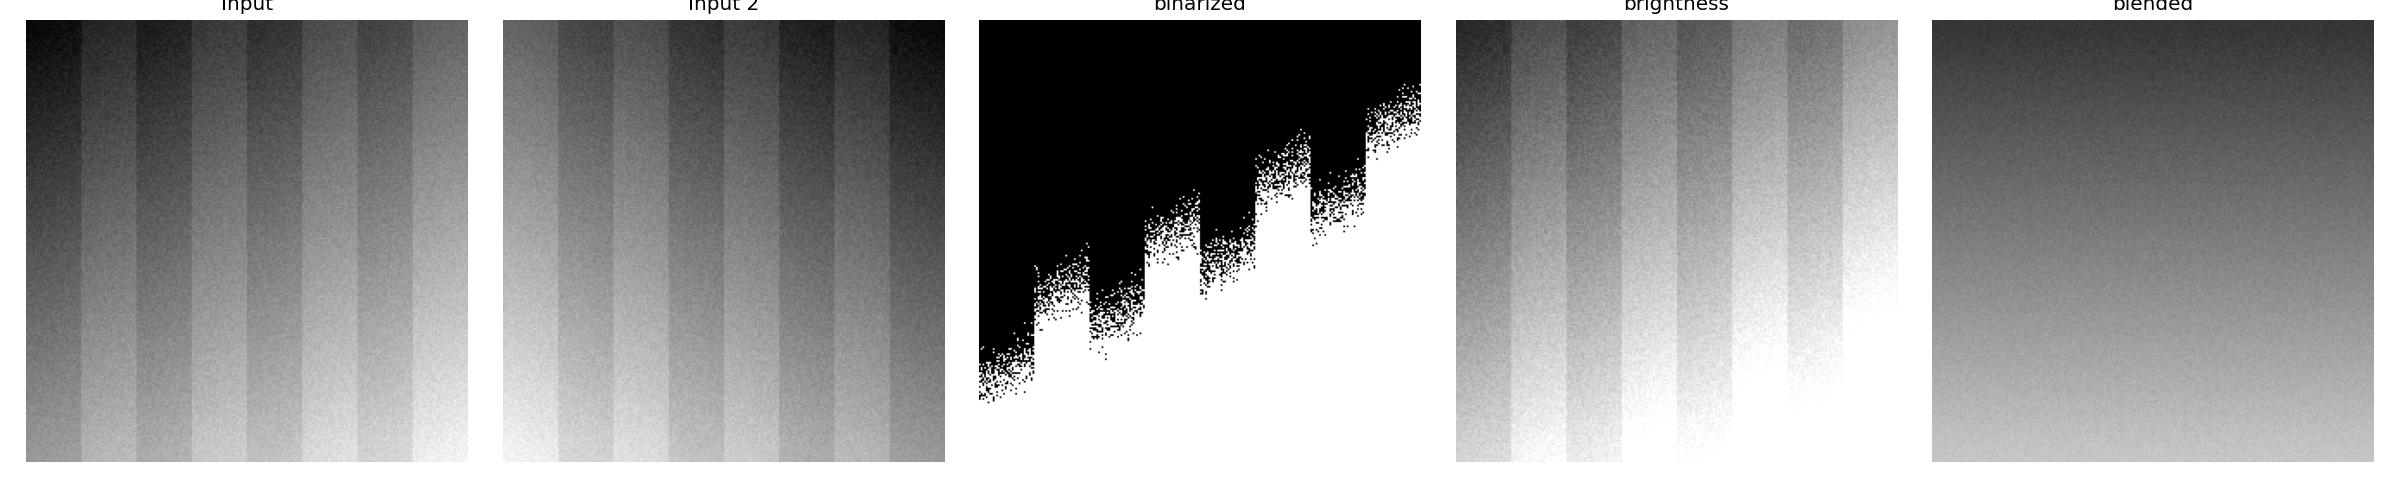
\includegraphics[width=1\linewidth,height=.25\textheight,keepaspectratio]{figures/images.png}
\end{center}

\section{Discussion}
The $32\times16$ block gave the lowest time for all three operations. Blending was slower than binarization and brightness in this run; it also reads two input images.

\end{document}
